% -*- coding: UTF-8 -*-
% vim: autoindent expandtab tabstop=4 sw=4 sts=4 filetype=tex
% vim: spelllang=de spell
% chktex-file 27 - disable warning about missing include files

\section{Komponenten}
\label{sec:main-components}

Ausgehend von den Anforderungen (\ref{sec:requirements}) können einzelne
Komponenten der Applikation abgeleitet werden. Einzelne Teile davon wurden
schon durch die Vision (\ref{sec:vision}) definiert beziehungsweise aus dieser
gewonnen.

Dieser Prozess entspricht nicht direkt dem Vorgehen
gemäss~\cite{larman_applying_2004} beziehungsweise dem UP, der Autor dieser
Projektarbeit ist jedoch der Ansicht, dass dieser Abschnitt eine Brücke
zwischen Anforderungen und der (Software-) Modellierung bildet. Zudem bietet
dieser Abschnitt eine relativ bildliche Beschreibung, was dem Verständnis des
Gesamtkonzeptes sicher zuträglich ist. Am ehesten entspricht dieser Abschnitt
den Komponenten-Diagrammen in~\cite[S. 653 bis 654]{larman_applying_2004}.

Die Applikation besteht aus zwei Applikationen: Einem \textit{Player},
welcher dem Abspielen von Echtzeit-Animationen dient, sowie einem \textit{Editor},
welcher der Erstellung und Verwaltung von Echtzeit-Animationen dient.

\subsection{Player}
\label{subsec:main-components:player}

Der \textit{Player} liest die vom \textit{Editor} exportierten
Echtzeit-Animationen. Er bietet vor dem Abspielen die Auswahl der Auflösung,
des Seitenverhältnisses, Antialiasing und ob die Animation im Vollbild-Modus
abgespielt werden soll.

\subsection{Editor}
\label{subsec:main-components:editor}

Der \textit{Editor} erlaubt das Erstellen und Bearbeiten von
Echtzeit-Animationen. Diese können schliesslich inklusive den
dazugehörigen Dateien, wie zum Beispiel Bitmaps oder Modellen, exportiert
werden.

\begin{figure}[h]
    \centering
    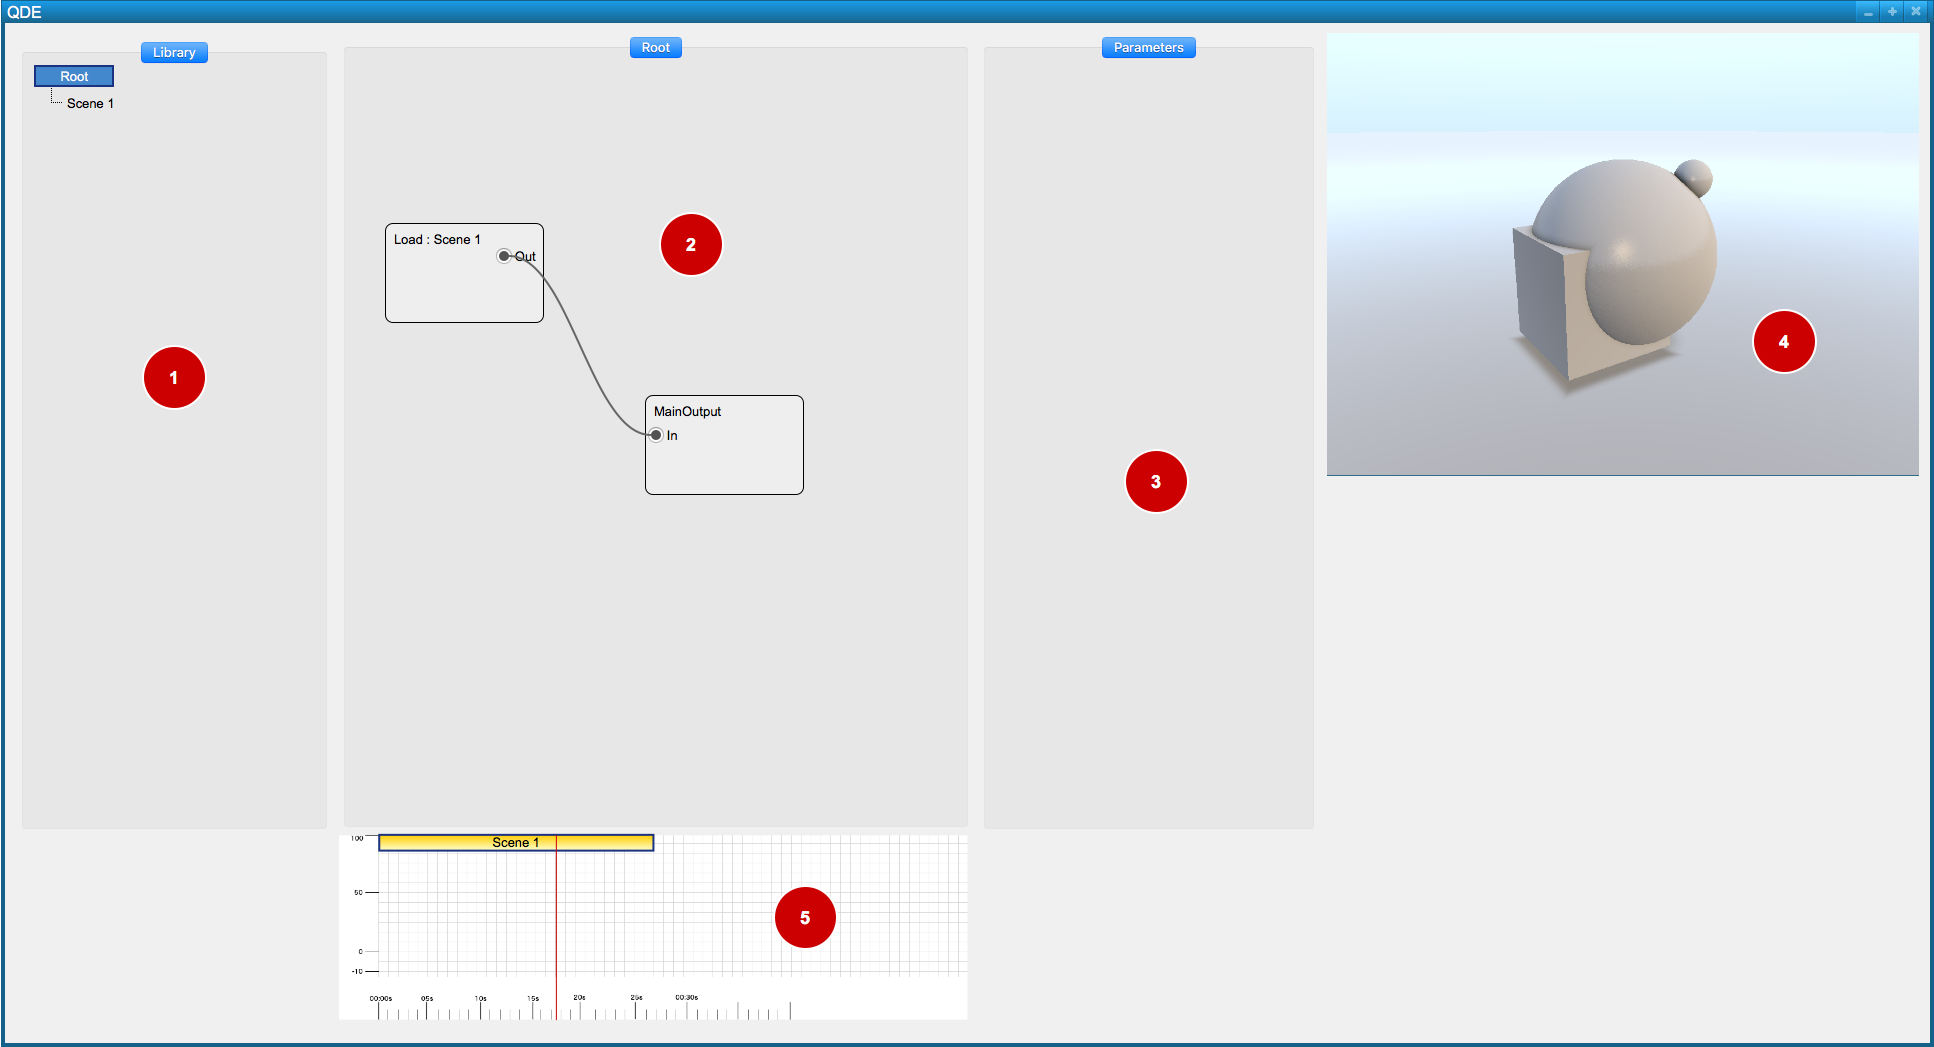
\includegraphics[width=0.9\textwidth]{img/editor_components.png}
    \caption{Einzelne Komponenten des Editors
        \protect\footnotemark}\label{fig:main-components:editor:editor-components}
\end{figure}
\footnotetext{Eigene Darstellung mittels Pencil.}

Abbildung~\ref{fig:main-components:editor:editor-components} zeigt die
einzelnen Komponenten des Editors. Nachfolgend findet sich eine Beschreibung
dieser.

\subsubsection{Bibliothek}
\label{ssubsec:main-components:editor:library}

Das Element~\img{img/editor_component_1.png} in
Abbildung~\ref{fig:main-components:editor:editor-components} zeigt die (Szenen-)
Bibliothek. Diese beinhaltet alle Szenen einer Echtzeit-Animation. Es können
neue Szenen angelegt und auch bestehende Szenen gelöscht werden. Wird ein neues
Projekt erstellt, so verfügt dieses immer über die ``Root''-Szene. Diese
beinhaltet den Haupt-Ausgabeknoten des Graphen
(\ref{ssubsec:main-components:editor:graph}), welcher schliesslich zum
Abspielen evaluiert wird, und kann nicht gelöscht werden. Wird eine Szene mit
der Maus angewählt, so wird deren Inhalt im Graphen
(\ref{ssubsec:main-components:editor:graph}) dargestellt.

\subsubsection{Graph}
\label{ssubsec:main-components:editor:graph}

Das Element~\img{img/editor_component_2.png} in
Abbildung~\ref{fig:main-components:editor:editor-components} zeigt den Graphen
einer Szene. Dieser beinhaltet sämtliche Knoten einer Szene. Mittels
Kontextmenü können neue Knoten eingefügt und bestehende Knoten gelöscht werden.
Wird ein Knoten angewählt, so wird dieser einerseits im
Rendering-Ansichtsfenster (\ref{ssubsec:main-components:editor:rendering})
dargestellt, andererseits werden dessen Eigenschaften im Parameter-Fenster
(\ref{ssubsec:main-components:editor:parameters}) angezeigt.

Folgende Typen von Knoten sind geplant:
\begin{itemize}
    \item{Scene}
    \item{TimelineClip}
    \item{Model}
    \item{Camera}
    \item{Light}
    \item{Material}
    \item{Operator}
    \item{Effect}
\end{itemize}

\subsubsection{Parameter}
\label{ssubsec:main-components:editor:parameters}

Das Element~\img{img/editor_component_3.png} in
Abbildung~\ref{fig:main-components:editor:editor-components} zeigt die Parameter
des aktuell gewählten Knoten im Graphen
(\ref{ssubsec:main-components:editor:graph}). Neben jedem Parameter befindet
sich eine Schaltfläche zum Setzen von Schlüsselbildern (Keyframes) in der
Zeitachse (Timeline,~\ref{ssubsec:main-components:editor:timeline}). Wird die
Schaltfläche betätigt, so wird bei dem aktuell ausgewählten Zeitpunkt der
Zeitachse ein Schlüsselbild gesetzt.

\subsubsection{Rendering}
\label{ssubsec:main-components:editor:rendering}

Das Element~\img{img/editor_component_4.png} in
Abbildung~\ref{fig:main-components:editor:editor-components} zeigt das
Rendering-Ansichtsfenster. Dieses stellt den Inhalt des aktuell gewählten
Knotens dar. Die Art des Knotens ist dabei nicht beschränkt, es kann dies eine
Szene, aber zum Beispiel auch ein einzelnes Modell sein. Es wird immer der
gesamte vorhergehende (Teil-) Baum des Knotens evaluiert.

\subsubsection{Zeitachse}
\label{ssubsec:main-components:editor:timeline}

Die Zeitachse wird mit~\img{img/editor_component_5.png} in
Abbildung~\ref{fig:main-components:editor:editor-scene1} dargestellt.  Sie
bildet das zeitliche Geschehen einer Echtzeit-Animation ab. Alle Knoten vom Typ
Timeline-Clip werden am oberen Rand des Fensters in deren zeitlicher
Reihenfolge abgebildet. Wird im Graph
(\ref{ssubsec:main-components:editor:graph}) ein Knoten mit animierten
Parametern (\ref{ssubsec:main-components:editor:parameters}) angewählt, so sind
diese ersichtlich. Vertikal wird der Wertebereich, horizontal die Zeitachse in
Sekunden dargestellt. Ein vertikal verlaufender, roter Marker zeigt die aktuelle
zeitliche Position der Echtzeit-Animation an.

Die untenstehende Abbildung~\ref{fig:main-components:editor:editor-scene1} zeigt ein Beispiel, wie eine typische Szene
mit animierten Parametern aussehen könnte.

\begin{figure}[H]
    \centering
    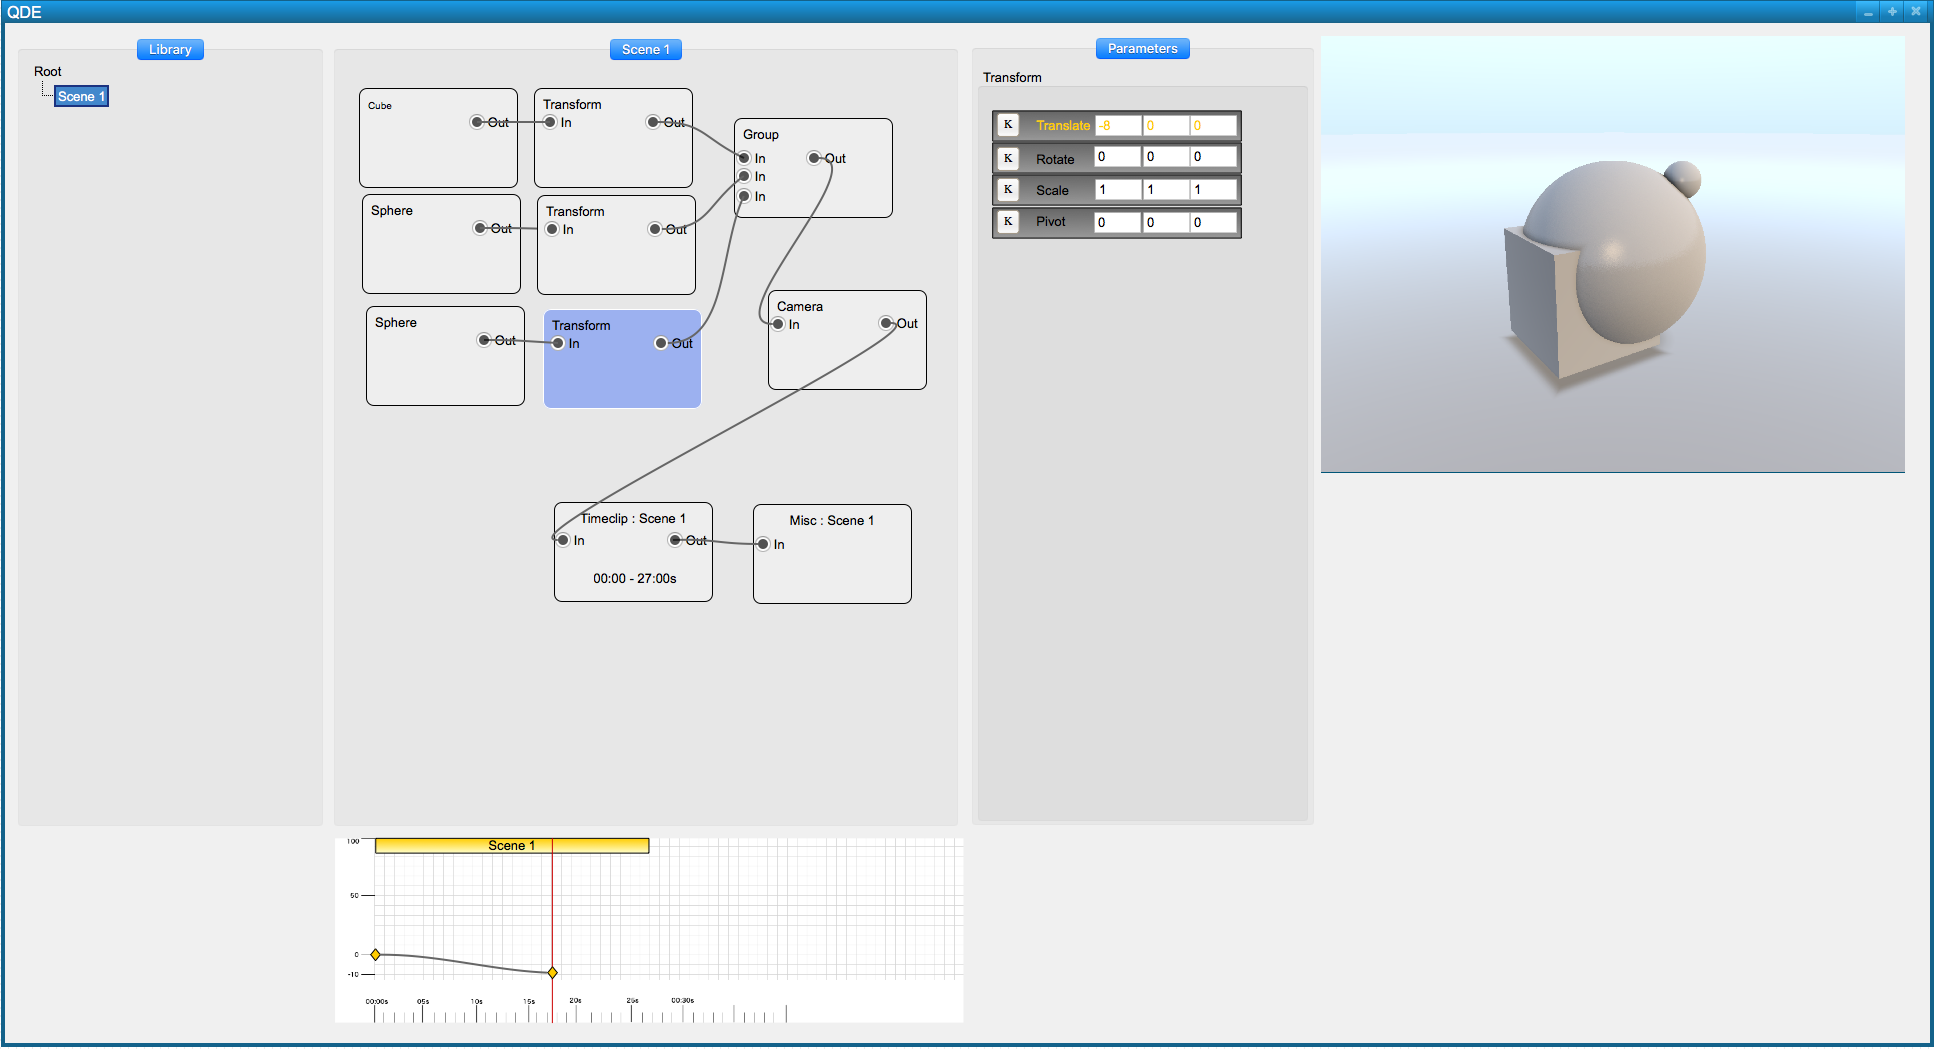
\includegraphics[width=0.9\textwidth]{img/editor_scene1.png}
    \caption{Beispiel-Szene innerhalb des Editors
        \protect\footnotemark}\label{fig:main-components:editor:editor-scene1}
\end{figure}
\footnotetext{Eigene Darstellung mittels Pencil.}
